\documentclass[]{beamer}
\usepackage{graphicx} 
\graphicspath{{Images/}{./}}
\usepackage{booktabs}
\usepackage{tikz}
\usepackage{pgfplots}
\usepackage{float}
\usepackage{listings,xcolor}

\usetheme{Madrid}
\usecolortheme{beaver}
\usefonttheme{default} 
\usepackage{palatino}
\usepackage[default]{opensans}
\useinnertheme{default}

\setbeamertemplate{footline}{}
\setbeamertemplate{navigation symbols}{}
\setbeamertemplate{headline}{}


\title[]{Zwischenpräsentation}

\author[shortname]{David Metzler \and Emircan Tutar  \and Niklas Kleiser}

\institute[shortinst]{ Hochschule Ravensburg Weingraten\\ \smallskip} 

\date{ \today}
%----------------------------------------------------------------------------------------

\begin{document}


%----------------------------------------------------------------------------------------
%	TITLE SLIDE
%----------------------------------------------------------------------------------------

\begin{frame}
	\titlepage % Output the title slide, automatically created using the text entered in the PRESENTATION INFORMATION block above
\end{frame}

%----------------------------------------------------------------------------------------
%	TABLE OF CONTENTS SLIDE
%----------------------------------------------------------------------------------------

% The table of contents outputs the sections and subsections that appear in your presentation, specified with the standard \section and \subsection commands. You may either display all sections and subsections on one slide with \tableofcontents, or display each section at a time on subsequent slides with \tableofcontents[pausesections]. The latter is useful if you want to step through each section and mention what you will discuss.

\begin{frame}
	\frametitle{Presentation Overview} % Slide title, remove this command for no title
	
	\tableofcontents % Output the table of contents (all sections on one slide)
	%\tableofcontents[pausesections] % Output the table of contents (break sections up across separate slides)
\end{frame}

%----------------------------------------------------------------------------------------
%	PRESENTATION BODY SLIDES
%----------------------------------------------------------------------------------------

\begin{frame}{Frame Title}

  \begin{figure}
    \begin{tikzpicture}[scale=0.]
		
		\draw [-, dashed, gray] (4,1)-- (-4,1)--(-4,3.5) --(4,3.5) --(4,1);
		
			\node at (-2.8 ,3) {BED VIEW};
					
		\node[inner sep=0pt] (whitehead) at (2,2.5)
		{
\includegraphics[width=.05\textwidth]{Images/camera.png}};
		
		\node[above] at (2.2,2.6) {\scriptsize Raspberry Pi und Kamera};
		
		\node[inner sep=0pt] (whitehead) at (0,2)
		{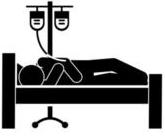
\includegraphics[width=.1\textwidth]{Images/person_in_bed.png}};

			\node at (-2.6 ,-1) {ROOM VIEW};
	
			\draw [-, dashed, gray] (4,-0.5)-- (-4,-0.5)--(-4,-4) --(4, -4 ) --(4,-0.5);
		
		\node[inner sep=0pt] (whitehead) at (2,-1.5)
		{
\includegraphics[width=.05\textwidth]{Images/camera.png}};
		

		
		\node[inner sep=0pt] (whitehead) at (-0.25,-1.25)
		{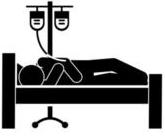
\includegraphics[width=.1\textwidth]{Images/person_in_bed.png}};
		
		
		\node[inner sep=0pt] (whitehead) at (0,-2.25)
		{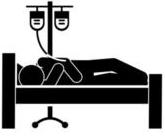
\includegraphics[width=.1\textwidth]{Images/person_in_bed.png}};
		
	\node[inner sep=0pt] (whitehead) at (-0.5,-3.25)
		{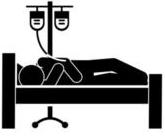
\includegraphics[width=.1\textwidth]{Images/person_in_bed.png}};
		

	  \node[inner sep=0pt] (whitehead) at (4.0,0.25)
		{
\includegraphics[width=.08\textwidth]{Images/server.png}};
		
				\node[below] at (2.2,-1.6) {\scriptsize Raspberry Pi und Kamera};
		
		\node[below] at (4.0,-0.1) {\scriptsize MQTT Broker};
		
			
		
		\draw [-] (2,2.5)-- ( 3,2.5) -- (3,0.25) ;
		\draw [-] (2,-1.5)-- ( 3,-1.5) -- (3,0.25) ;
		\draw [-]  (3,0.25)  -- (3.8,0.25);

	    \draw [->]  (4.2 ,0.25) -- (5.0,0.25) -- (5.0,-1.5) -- (5.5,-1.5);
	     \draw [->]  (4.2 ,0.25) -- (5.0,0.25) -- (5.0,2.5) -- (5.5,2.5);
	
		\node at  (7.0,2.5) {Bed Detection};
		
		
		\node at  (7.0,-1.5) {Fall Detection};
		
		
	
	 	\draw [->]  (8.5 ,-1.5) -- (9.0,-1.5) -- (9,0.25) -- (9.5,0.25)  ;
	
		\draw [->]  (8.5, 2.5) -- (9.0,2.5) -- (9,0.25) -- (9.5,0.25) ;
		
		\node[inner sep=0pt] (whitehead) at (9.85,0.25)
		{
\includegraphics[width=.05\textwidth]{Images/raspi.png}};
		
		\node[below] at (10.,0.1) {\scriptsize Raspberry Pi };
		
		\draw [->]  (10.3,0.25) -- (10.6,0.25) ;
		
		\node[red] at  (11.2,0.25) {Alarm};
		
		
	\end{tikzpicture}

    \caption{Systemaufbau}
  \end{figure}

    
\end{frame}

\section{Lastenheft}
\subsection{Muss - Anforderungen}
\begin{frame}
\frametitle{Lastenheft}
\framesubtitle{Muss - Anforderungen}
\begin{enumerate}
    \item Docker
    \item Ubuntu 22.04 (LTS)
    \item Dynamisches DNS-Management (ddclient)
    \item Fail2ban
    \item MQTT / MQTT-Client
    \item SMTP-Server / SMTP-Client
    \item Raspberry und Raspberry Pi
    \item Fall Detektion
    \item Matrix
\end{enumerate}
\end{frame}

\subsection{Soll - Anforderungen}
\begin{frame}
\frametitle{Lastenheft}
\framesubtitle{Soll - Anforderungen}
\begin{enumerate}
    \item Bett Detektion
    \item Alarm (Ton und Licht)
    \item Firewall
\end{enumerate}
\end{frame}

\subsection{Kann - Anforderungen}
\begin{frame}
\frametitle{Lastenheft}
\framesubtitle{Kann - Anforderungen}
\begin{enumerate}
    \item MQTT Frontend
    \item Gesprochene Information über Patient in Hilfesituation
    \item Kameraview
\end{enumerate}
\end{frame}

%------------------------------------------------

\section{Referencing}

\begin{frame}
	\frametitle{Citing References}
	
	An example of the \texttt{\textbackslash cite} command to cite within the presentation:
	
	\bigskip % Vertical whitespace
	
	This statement requires citation \cite{p1,p2}.
\end{frame}

%------------------------------------------------

\begin{frame} % Use [allowframebreaks] to allow automatic splitting across slides if the content is too long
	\frametitle{References}
	
	\begin{thebibliography}{99} % Beamer does not support BibTeX so references must be inserted manually as below, you may need to use multiple columns and/or reduce the font size further if you have many references
		\footnotesize % Reduce the font size in the bibliography
		
		\bibitem[Smith, 2022]{p1}
			John Smith (2022)
			\newblock Publication title
			\newblock \emph{Journal Name} 12(3), 45 -- 678.
			
		\bibitem[Kennedy, 2023]{p2}
			Annabelle Kennedy (2023)
			\newblock Publication title
			\newblock \emph{Journal Name} 12(3), 45 -- 678.
	\end{thebibliography}
\end{frame}

%----------------------------------------------------------------------------------------
%	ACKNOWLEDGMENTS SLIDE
%----------------------------------------------------------------------------------------

\begin{frame}
	\frametitle{Acknowledgements}
	
	\begin{columns}[t] % The "c" option specifies centered vertical alignment while the "t" option is used for top vertical alignment
		\begin{column}{0.45\textwidth} % Left column width
			\textbf{Smith Lab}
			\begin{itemize}
				\item Alice Smith
				\item Devon Brown
			\end{itemize}
			\textbf{Cook Lab}
			\begin{itemize}
				\item Margaret
				\item Jennifer
				\item Yuan
			\end{itemize}
		\end{column}		
		\begin{column}{0.5\textwidth} % Right column width
			\textbf{Funding}
			\begin{itemize}
				\item British Royal Navy
				\item Norwegian Government
			\end{itemize}
		\end{column}
	\end{columns}
\end{frame}

%----------------------------------------------------------------------------------------
%	CLOSING SLIDE
%----------------------------------------------------------------------------------------

\begin{frame}[plain] % The optional argument 'plain' hides the headline and footline
	\begin{center}
		{\Huge The End}
		
		\bigskip\bigskip % Vertical whitespace
		
		{\LARGE Questions? Comments?}
	\end{center}
\end{frame}

%----------------------------------------------------------------------------------------

\end{document} 